% The document class supplies options to control rendering of some standard
% features in the result.  The goal is for uniform style, so some attention 
% to detail is *vital* with all fields.  Each field (i.e., text inside the
% curly braces below, so the MEng text inside {MEng} for instance) should 
% take into account the following:
%
% - author name       should be formatted as "FirstName LastName"
%   (not "Initial LastName" for example),
% - supervisor name   should be formatted as "Title FirstName LastName"
%   (where Title is "Dr." or "Prof." for example),
% - degree programme  should be "BSc", "MEng", "MSci", "MSc" or "PhD",
% - dissertation title should be correctly capitalised (plus you can have
%   an optional sub-title if appropriate, or leave this field blank),
% - dissertation type should be formatted as one of the following:
%   * for the MEng degree programme either "enterprise" or "research" to
%     reflect the stream,
%   * for the MSc  degree programme "$X/Y/Z$" for a project deemed to be
%     X%, Y% and Z% of type I, II and III.
% - year              should be formatted as a 4-digit year of submission
%   (so 2014 rather than the academic year, say 2013/14 say).

\documentclass[ % the name of the author
                    author={Manan Vaswani},
                % the name of the supervisor
                supervisor={Dr. Raphael Clifford},
                % the degree programme
                    degree={MEng},
                % the dissertation    title (which cannot be blank)
                     title={A multi-core CPU implementation \n of the classical Boson Sampling algorithm},
                % the dissertation subtitle (which can    be blank)
                  subtitle={},
                % the dissertation     type
                      type={},
                % the year of submission
                      year={2019} ]{dissertation}

\begin{document}

% =============================================================================

% This section simply introduces the structural guidelines.  It can clearly
% be deleted (or commented out) if you use the file as a template for your
% own dissertation: everything following it is in the correct order to use 
% as is.

% =============================================================================

% This macro creates the standard UoB title page by using information drawn
% from the document class (meaning it is vital you select the correct degree 
% title and so on).

\maketitle

% After the title page (which is a special case in that it is not numbered)
% comes the front matter or preliminaries; this macro signals the start of
% such content, meaning the pages are numbered with Roman numerals.

\frontmatter

% This macro creates the standard UoB declaration; on the printed hard-copy,
% this must be physically signed by the author in the space indicated.

\makedecl

% LaTeX automatically generates a table of contents, plus associated lists 
% of figures, tables and algorithms.  The former is a compulsory part of the
% dissertation, but if you do not require the latter they can be suppressed
% by simply commenting out the associated macro.

\tableofcontents
%\listoffigures
%\listoftables
%\listofalgorithms
%\lstlistoflistings

% The following sections are part of the front matter, but are not generated
% automatically by LaTeX; the use of \chapter* means they are not numbered.

% -----------------------------------------------------------------------------

\chapter*{Executive Summary}

{\bf A compulsory section, of at most $1$ page} 
\vspace{1cm} 

\noindent
This section should pr\'{e}cis the project context, aims and objectives,
and main contributions (e.g., deliverables) and achievements; the same 
section may be called an abstract elsewhere.  The goal is to ensure the 
reader is clear about what the topic is, what you have done within this 
topic, {\em and} what your view of the outcome is.

The former aspects should be guided by your specification: essentially 
this section is a (very) short version of what is typically the first 
chapter.  Note that for research-type projects, this {\bf must} include 
a clear research hypothesis.  This will obviously differ significantly
for each project, but an example might be as follows:

\begin{quote}
My research hypothesis is that a suitable genetic algorithm will yield
more accurate results (when applied to the standard ACME data set) than 
the algorithm proposed by Jones and Smith, while also executing in less
time.
\end{quote}

\noindent
The latter aspects should (ideally) be presented as a concise, factual 
bullet point list.  Again the points will differ for each project, but 
an might be as follows:

\begin{quote}
\noindent
\begin{itemize}
\item I spent $120$ hours collecting material on and learning about the 
      Java garbage-collection sub-system. 
\item I wrote a total of $5000$ lines of source code, comprising a Linux 
      device driver for a robot (in C) and a GUI (in Java) that is 
      used to control it.
\item I designed a new algorithm for computing the non-linear mapping 
      from A-space to B-space using a genetic algorithm, see page $17$.
\item I implemented a version of the algorithm proposed by Jones and 
      Smith in [6], see page $12$, corrected a mistake in it, and 
      compared the results with several alternatives.
\end{itemize}
\end{quote}


% -----------------------------------------------------------------------------

\chapter*{Supporting Technologies}

{\bf A compulsory section, of at most $1$ page}
\vspace{1cm} 

\noindent
This section should present a detailed summary, in bullet point form, 
of any third-party resources (e.g., hardware and software components) 
used during the project.  Use of such resources is always perfectly 
acceptable: the goal of this section is simply to be clear about how
and where they are used, so that a clear assessment of your work can
result.  The content can focus on the project topic itself (rather,
for example, than including ``I used \mbox{\LaTeX} to prepare my 
dissertation''); an example is as follows:

\begin{quote}
\noindent
\begin{itemize}
\item I used the Java {\tt BigInteger} class to support my implementation 
      of RSA.
\item I used a parts of the OpenCV computer vision library to capture 
      images from a camera, and for various standard operations (e.g., 
      threshold, edge detection).
\item I used an FPGA device supplied by the Department, and altered it 
      to support an open-source UART core obtained from 
      \url{http://opencores.org/}.
\item The web-interface component of my system was implemented by 
      extending the open-source WordPress software available from
      \url{http://wordpress.org/}.
\end{itemize}
\end{quote}

% -----------------------------------------------------------------------------

\chapter*{Acknowledgements}

{\bf An optional section, of at most $1$ page}
\vspace{1cm} 

\noindent
I would like to thank my supervisor, Dr. Raphael Clifford, for his help and support throughout the year and for introducing me to the Boson Sampling problem.

% =============================================================================

% After the front matter comes a number of chapters; under each chapter,
% sections, subsections and even subsubsections are permissible.  The
% pages in this part are numbered with Arabic numerals.  Note that:
%
% - A reference point can be marked using \label{XXX}, and then later
%   referred to via \ref{XXX}; for example Chapter\ref{chap:context}.
% - The chapters are presented here in one file; this can become hard
%   to manage.  An alternative is to save the content in seprate files
%   the use \input{XXX} to import it, which acts like the #include
%   directive in C.

\mainmatter

% -----------------------------------------------------------------------------

\chapter{Contextual Background}
\label{chap:context}

{\bf A compulsory chapter,     of roughly $5$ pages}
\vspace{1cm} 

\noindent
The advances made in the field of quantum algorithms in the past 25 years has given rise to questions about whether a number of classical hypotheses still hold true in light of modern quantum research The most notable example is the Extended Church-Turing Thesis which in simple terms says that all computational problems that are efficiently solvable by realistic physical devices are efficiently solvable by a probabilistic Turing machine \cite{kaye2007}. However, Shor's algorithm \cite{shor1995} potentially disproves this. Informally, Shor's discovery stated that if a classical computer could accurately simulate a quantum-mechanical experiment in probabilisitic polynomial time, then it must be able to factor integers in polynomial time as well. The problem of factoring integers is known to have no polynomial-time algorithm on a classical computer. It is so widely accepted that factoring integers is a hard problem that a number of cryptographic systems are built on its hardness, including the famous RSA algorithm \cite{rsa1978}. Hence, Shor's algorithm has a strong implication: A classical computer that is able to simulate quantum experiments efficiently, it would be able to break widely used cryptosystems such as RSA.

The topic of classically simulating quantum systems is a central idea in the field of quantum supremacy. Quantum supremacy is the phenomena that there exist quantum experiments that cannot be accurately and efficiently simulated using classical systems. Numerous attempts have been made to demonstrate quantum supremacy but the current physical limitations of quantum systems has made that an extremely challenging problem. Additionally, what makes it so hard to demonstrate is that it is not defined in terms of the ability of a quantum system to solve a particular problem, but rather it requires showing that classical computers cannot solve a problem. In a way, it could be likened to classifying computational problems into complexity classes \cite{papadimitriou2003}. In the same way that a number of complexity theory related theorems and conjectures rely on a number of theoretic assumptions, it is necessary for quantum supremacy to rely on similar such assumptions as well, as it would be nearly impossible to unconditionally prove such statements \cite{harrow2017}.

Linking back to Shor's algorithm and its potential to demonstrate quantum supremacy and simultaneously disprove the Extended-Church Turing thesis, there are two significant drawbacks which prevent it from doing so. 

Firstly, the problem of factoring integers, while widely believed to be an $\NP-\text{hard}$ problem, its hardness has not been formally proved. The assumption is not strong enough to verify that Shor's algorithm does achieve quantum supremacy.

The second, and more obvious drawback with Shor's algorithm is that a large-scale physical implementation of a quantum computer to run it is beyond the current reach of technology. While there have been several experiments that successfully factor small numbers like 15 \cite{monz2016} and 21 \cite{vartiainen2004} with high accuracy, we are not at risk of RSA breaking just yet!

This has motivated the search for other such quantum experiments that can be run physically, but not simulated classically. However, and important requirement is that it should be possible to model these experiments as computational problems in order to compare the hardness.

There are a handful of problems that satisfy this criteria, such as the problem of sampling the output distribution of random quantum circuits, which has been one of the most popular problems in the field of quantum supremacy in the past few years due to a lot of interest from big companies like Google and IBM. The best known classical algorithm for simulating the task of sampling bitstrings from the output of random quantum circuits is exponential in the number of qubits in the bitstring, leading one group of researchers in 2016 to estimate that a physical experiment with $\approx 50$ qubits could be enough to demonstrate quantum supremacy \cite{boixo2016}. However, more recently a classical simulation of the problem with 56 qubits was carried out successfully \cite{pednault2017}. This pushed the imminence of quantum supremacy for the circuit sampling problem even further away.

The other famous problem in the field of quantum supremacy, of a similar flavour, is the Boson Sampling problem, which is the main focus of this paper. While the problem reduces down to a sampling problem like circuit sampling, as the name suggests, it actually belongs to a paradigm of Quantum Computation different to the ones discussed before, called Linear Optical Quantum Computation (or LOQC). The protocol by Knill, Laflamme and Milburn in 2001 \cite{knill2001} demonstrated that a scalable quantum computer with linear optical elements could be robustly implemented. In LOQC, a photon is used to represent a single qubit.

Aaronson and Arkhipov in their paper on the classical complexity of linear optics showed that it was possible to build a quantum computation model within the LOQC paradigm which could not be efficiently simulated by classical computers \cite{aaronson2011}. They define a model for `Boson Sampling' in which $n$ identical photons are passed through a linear optical network and then measured to determine their location. This linear optical network consists of a collection of simple optical elements called beam splitters and phase shifters.

\begin{figure}
	\centering
  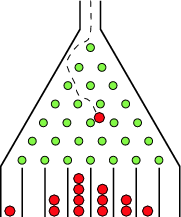
\includegraphics[width=15em]{galton_board}
  \caption{A Galton board, used to demonstrate sampling from a binomial distribution \cite{galton_board}}
  \label{fig:galton_board}
\end{figure}

The model could be thought of as being a parallel to a Galtons Board, shown in figure \ref{fig:galton_board}, in which $n$ balls are dropped into a vertical lattice of wooden pegs, each of which randomly scatters an incoming ball to one of two other pegs with equal probability. The input to this system is the exact arrangement of the pegs, while the output is the number of balls that have landed at each location on the bottom. The output could alternatively be thought of as a sample from the distribution of all possible output arrangements (which is the binomial distribution in this case).

In the Aaronson and Arkhipovs Boson Sampling model, the balls are replaced with identical photons, and the pegs arranged in a lattice are replaced with an arbitrary arrangement of optical elements. Also, the photons can be dropped from different starting locations as opposed to just a single position. The Boson-Sampling problem involves sampling the output distribution using photon-number discriminating detectors. They argued that if there is a polynomial time classical algorithm that exactly samples from the Boson Sampling distribution, the complexity class $\P^{\#\P} = \BPP^{\NP} $  which would collapse the polynomial hierarchy to the third level by Toda's theorem \cite{toda1991}.

In order to actually compare the physical model with a classical computational model, the paper reduces the Boson Sampling problem to a problem in purely mathematical terms. Photons are a type of boson, which is one of the two main types of particles in the world. The link between bosons and permanents of matrices has been known since 1953, from the work by Caianiello \cite{Caianiello1953} which showed that the amplitudes of $n$-boson process can be written as the permanents of $n \times n$ matrices. Hence it was possible to represent the Boson Sampling distribution in terms of the permanents of matrices, and this was shown and proved in the paper.

Carrying out a physical experiment for Boson Sampling is not a trivial task, and increasing the number of photons or the number of output modes to large enough values is extremely difficult. The current experimental record is with 5 photons and 9 output modes. However, this does show the possibility of potentially having larger-scale implementations in the future.

The Aaronson and Arkhipov paper provoked much interest in the classical computation algorithm for Boson Sampling. Much of the work is focussed around fast implementations for the calculation of permanents of large matrices, with recent works showing efficient results for matrices as large as $54 \times 54$ \cite{roga2019, lundow2019}. There have been a few other approaches to simulating the Boson sampling problem such as classically modelling the Linear optical network itself, and sampling from the output as opposed to computing the purely mathematical equivalent of the problem \cite{rahimi2016}. There have also been attempts at using Markov Chain Monte Carlo (MCMC) methods to sample from the Boson Sampling distribution by trying to identify it as the equilibrium distribution of a Markov chain, following the method by Hastings \cite{hastings1970}. However, estimating how accurately these methods approximate to the true Boson Sampling experiment has been difficult. Nonetheless, the MCMC method proposed by Neville et. al. \cite{neville2017} gave strong numerical evidence that classical Boson Sampling may be feasible for large input sizes.

In terms of actual implementations of the Boson Sampling algorithm, there have been few, with the most significant benchmark being the test of the simulation run on the Tianhe-2 supercomputer \cite{wu2018} which managed to simulate Boson Sampling for 50 photons with a runtime of approximately 100 minutes.

However, in the groundbreaking paper by Clifford and Clifford \cite{clifford17}, a new significantly faster algorithm was proposed which showed promise of carrying out classical Boson Sampling in an even shorter time. The algorithm proposed in this paper is central to our work. We give a highly optimised implementation of this algorithm with the aim of setting a new benchmark for the classical Boson Sampling problem, and in the process pushing away the imminence of quantum supremacy in the near future.


\begin{quote}
\noindent
The high-level objective of this project is to reduce the performance 
gap between hardware and software implementations of modular arithmetic.  
More specifically, the concrete aims are:

\begin{enumerate}
\item Research and survey literature on public-key cryptography and
      identify the state of the art in exponentiation algorithms.
\item Improve the state of the art algorithm so that it can be used
      in an effective and flexible way on constrained devices.
\item Implement a framework for describing exponentiation algorithms
      and populate it with suitable examples from the literature on 
      an ARM7 platform.
\item Use the framework to perform a study of algorithm performance
      in terms of time and space, and show the proposed improvements
      are worthwhile.
\end{enumerate}
\end{quote}

% -----------------------------------------------------------------------------

\chapter{Technical Background}
\label{chap:technical}

{\bf A compulsory chapter,     of roughly $10$ pages} 
\vspace{1cm} 

\noindent
This chapter is intended to describe the technical basis on which execution
of the project depends.  The goal is to provide a detailed explanation of
the specific problem at hand, and existing work that is relevant (e.g., an
existing algorithm that you use, alternative solutions proposed, supporting
technologies).  

Per the same advice in the handbook, note there is a subtly difference from
this and a full-blown literature review (or survey).  The latter might try
to capture and organise (e.g., categorise somehow) {\em all} related work,
potentially offering meta-analysis, whereas here the goal is simple to
ensure the dissertation is self-contained.  Put another way, after reading 
this chapter a non-expert reader should have obtained enough background to 
understand what {\em you} have done (by reading subsequent sections), then 
accurately assess your work.  You might view an additional goal as giving 
the reader confidence that you are able to absorb, understand and clearly 
communicate highly technical material.

% -----------------------------------------------------------------------------

\chapter{Project Execution}
\label{chap:execution}

{\bf A topic-specific chapter, of roughly $15$ pages} 
\vspace{1cm} 

\noindent
This chapter is intended to describe what you did: the goal is to explain
the main activity or activities, of any type, which constituted your work 
during the project.  The content is highly topic-specific, but for many 
projects it will make sense to split the chapter into two sections: one 
will discuss the design of something (e.g., some hardware or software, or 
an algorithm, or experiment), including any rationale or decisions made, 
and the other will discuss how this design was realised via some form of 
implementation.  

This is, of course, far from ideal for {\em many} project topics.  Some
situations which clearly require a different approach include:

\begin{itemize}
\item In a project where asymptotic analysis of some algorithm is the goal,
      there is no real ``design and implementation'' in a traditional sense
      even though the activity of analysis is clearly within the remit of
      this chapter.
\item In a project where analysis of some results is as major, or a more
      major goal than the implementation that produced them, it might be
      sensible to merge this chapter with the next one: the main activity 
      is such that discussion of the results cannot be viewed separately.
\end{itemize}

\noindent
Note that it is common to include evidence of ``best practice'' project 
management (e.g., use of version control, choice of programming language 
and so on).  Rather than simply a rote list, make sure any such content 
is useful and/or informative in some way: for example, if there was a 
decision to be made then explain the trade-offs and implications 
involved.

\section{Example Section}

This is an example section; 
the following content is auto-generated dummy text.
\lipsum

\subsection{Example Sub-section}

\begin{figure}[t]
\centering
foo
\caption{This is an example figure.}
\label{fig}
\end{figure}

\begin{table}[t]
\centering
\begin{tabular}{|cc|c|}
\hline
foo      & bar      & baz      \\
\hline
$0     $ & $0     $ & $0     $ \\
$1     $ & $1     $ & $1     $ \\
$\vdots$ & $\vdots$ & $\vdots$ \\
$9     $ & $9     $ & $9     $ \\
\hline
\end{tabular}
\caption{This is an example table.}
\label{tab}
\end{table}

\begin{algorithm}[t]
\For{$i=0$ {\bf upto} $n$}{
  $t_i \leftarrow 0$\;
}
\caption{This is an example algorithm.}
\label{alg}
\end{algorithm}

\begin{lstlisting}[float={t},caption={This is an example listing.},label={lst},language=C]
for( i = 0; i < n; i++ ) {
  t[ i ] = 0;
}
\end{lstlisting}

This is an example sub-section;
the following content is auto-generated dummy text.
Notice the examples in Figure~\ref{fig}, Table~\ref{tab}, Algorithm~\ref{alg}
and Listing~\ref{lst}.
\lipsum

\subsubsection{Example Sub-sub-section}

This is an example sub-sub-section;
the following content is auto-generated dummy text.
\lipsum

\paragraph{Example paragraph.}

This is an example paragraph; note the trailing full-stop in the title,
which is intended to ensure it does not run into the text.

% -----------------------------------------------------------------------------

\chapter{Critical Evaluation}
\label{chap:evaluation}

{\bf A topic-specific chapter, of roughly $15$ pages} 
\vspace{1cm} 

\noindent
This chapter is intended to evaluate what you did.  The content is highly 
topic-specific, but for many projects will have flavours of the following:

\begin{enumerate}
\item functional  testing, including analysis and explanation of failure 
      cases,
\item behavioural testing, often including analysis of any results that 
      draw some form of conclusion wrt. the aims and objectives,
      and
\item evaluation of options and decisions within the project, and/or a
      comparison with alternatives.
\end{enumerate}

\noindent
This chapter often acts to differentiate project quality: even if the work
completed is of a high technical quality, critical yet objective evaluation 
and comparison of the outcomes is crucial.  In essence, the reader wants to
learn something, so the worst examples amount to simple statements of fact 
(e.g., ``graph X shows the result is Y''); the best examples are analytical 
and exploratory (e.g., ``graph X shows the result is Y, which means Z; this 
contradicts [1], which may be because I use a different assumption'').  As 
such, both positive {\em and} negative outcomes are valid {\em if} presented 
in a suitable manner.

% -----------------------------------------------------------------------------

\chapter{Conclusion}
\label{chap:conclusion}

{\bf A compulsory chapter,     of roughly $5$ pages} 
\vspace{1cm} 

\noindent
The concluding chapter of a dissertation is often underutilised because it 
is too often left too close to the deadline: it is important to allocation
enough attention.  Ideally, the chapter will consist of three parts:

\begin{enumerate}
\item (Re)summarise the main contributions and achievements, in essence
      summing up the content.
\item Clearly state the current project status (e.g., ``X is working, Y 
      is not'') and evaluate what has been achieved with respect to the 
      initial aims and objectives (e.g., ``I completed aim X outlined 
      previously, the evidence for this is within Chapter Y'').  There 
      is no problem including aims which were not completed, but it is 
      important to evaluate and/or justify why this is the case.
\item Outline any open problems or future plans.  Rather than treat this
      only as an exercise in what you {\em could} have done given more 
      time, try to focus on any unexplored options or interesting outcomes
      (e.g., ``my experiment for X gave counter-intuitive results, this 
      could be because Y and would form an interesting area for further 
      study'' or ``users found feature Z of my software difficult to use,
      which is obvious in hindsight but not during at design stage; to 
      resolve this, I could clearly apply the technique of Smith [7]'').
\end{enumerate}

% =============================================================================

% Finally, after the main matter, the back matter is specified.  This is
% typically populated with just the bibliography.  LaTeX deals with these
% in one of two ways, namely
%
% - inline, which roughly means the author specifies entries using the 
%   \bibitem macro and typesets them manually, or
% - using BiBTeX, which means entries are contained in a separate file
%   (which is essentially a databased) then inported; this is the 
%   approach used below, with the databased being dissertation.bib.
%
% Either way, the each entry has a key (or identifier) which can be used
% in the main matter to cite it, e.g., \cite{X}, \cite[Chapter 2}{Y}.

\backmatter

\bibliography{dissertation}

% -----------------------------------------------------------------------------

% The dissertation concludes with a set of (optional) appendicies; these are 
% the same as chapters in a sense, but once signaled as being appendicies via
% the associated macro, LaTeX manages them appropriatly.

\appendix

\chapter{An Example Appendix}
\label{appx:example}

Content which is not central to, but may enhance the dissertation can be 
included in one or more appendices; examples include, but are not limited
to

\begin{itemize}
\item lengthy mathematical proofs, numerical or graphical results which 
      are summarised in the main body,
\item sample or example calculations, 
      and
\item results of user studies or questionnaires.
\end{itemize}

\noindent
Note that in line with most research conferences, the marking panel is not
obliged to read such appendices.

% =============================================================================

\end{document}
